%=========================================================================
% (c) 2014, 2015 Josef Lusticky

\subsection{Receive offloads}\label{subsec:linux-ingress-offloads}
Network adapter vendors have been adding protocol support to their cards.
This support can vary from the simple (checksumming of packets, for example)
through to full TCP/IP implementations~\cite{linux-and-tcp-offload-engines}.

To mitigate CPU load spent on TCP overhead completely, the TCP Offload Engine (TOE) is implemented in several NICs.
TOE features a full TCP/IP implementation in adapter, including the TCP connection management.
However, Linux has never supported the TOE features of any network cards~\cite{linux-and-tcp-offload-engines}.
Vendors have made modifications to the Linux kernel to support TOE,
and these changes have been submitted for kernel inclusion but were rejected~\cite{linux-foundation-toe}. 

Linux kernel engineers currently feel that the full network stack offload
that TOE provides has little merit~\cite{linux-foundation-toe}.
TOE shorts out much of the Linux networking code, described in the previous sections.
In the process, it cuts out features like netfilter, traffic control, and more.
The Linux networking stack is easy to fix when a bug or security issue comes up~\cite{linux-and-tcp-offload-engines}.
If a security problem turns up in a TOE adapter, instead, there is very little which can be done to fix it.
Linux engineers claim that 100~Mbps TOE adapters
(which used to be the bleeding-edge high speed)
are now slower than the Linux networking stack.
So any performance advantage from TOE is a temporary thing, but once the TOE's code is merged, it must be supported.
As a result of this, TOE support might become a long-term maintenance burden~\cite{linux-and-tcp-offload-engines}.

Although inclusion of TOE support was rejected, there are ways to obtain TOE's performance without
necessitating stateful support in the cards~\cite{linux-and-tcp-offload-engines}.
Everything that is worthwhile can be done with stateless offloads.
One of the simplest stateless offload technique is computing checksums in hardware.
With receive (Rx) checksum offload, IP, TCP and UDP checksums are checked in the hardware of the NIC upon frame reception.

While checksum offload provides some performance improvement,
a large portion of per-packet processing overhead remains.
Each packet is passed through the entire IP stack, as described in section~\ref{sec:linux-ip}.
Dealing with each single packet takes a significant amount of the CPU time, particularly on high-speed Ethernet links that
can produce millions of packets per second.

Given the importance of per-packet overhead, it makes sense to raise the MTU.
However, most connections of interest go across the Internet,
and those are all bound by the lowest MTU in the entire path.
As noted in section~\ref{sec:40gbe-compatibility}, the IEEE has determined no support for frames with MTU larger than 1500.
Protocol-based mechanisms for MTU discovery exist, but they do not work well on the Internet,
because in particular, a lot of firewall setups do not allow them to work~\cite{jls2009-gro}.

If the kernel can not use a larger MTU, it can pretend that it is using a larger MTU.
An optimisation technique to pretend larger MTU is provided by the Large Receive Offload (LRO).
LRO merges packets of the same TCP flow together,
creating one large super-frame, before it is passed to the higher network layers~\cite{jls2009-gro}.
Merging multiple packets and processing them as a single packet
reduces CPU overhead and thus improves performance~\cite{linux-kernel-networking}.
The merging can be done either in the driver or in the hardware.
Even LRO emulation in the driver has performance benefits~\cite{jls2009-gro}.

Since LRO merges everything of the same TCP flow into one large super-frame,
the differences in the headers of these packets are lost~\cite{jls2009-gro}.
If a system is acting as a router, it should not be changing the headers on packets as they pass through,
because it brakes the end-to-end principle and can significantly impact performance~\cite{linux-kernel-networking}.

A generic solution was introduced by the Generic Receive Offload (GRO) to mitigate the problems of LRO.
In GRO, the criteria for which packets can be merged is greatly restricted.
The MAC headers must be identical and only a few TCP or IP headers can differ -
checksums are necessarily different and the Identification field is allowed to increment~\cite{jls2009-gro}.
As a result of these restrictions, merged packets can be later resegmented losslessly
and therefore the GRO feature can be used by a system
acting as a router without braking the end-to-end principle~\cite{jls2009-gro}.
However, GRO still requires the L4 protocol to have its own segmentation support
and it is currently restricted to TCP only~\cite{linux-kernel-networking}.

When using GRO, merging packets of the same flow into one large super-frame must be time-limited.
In combination with NAPI, there is no need for any special waiting code -
the kernel already calls the driver's poll method for new packets occasionally and processes them in batches.
Thus, GRO can simply be performed at NAPI poll time without introducing any additional latency~\cite{jls2009-gro}.
The GRO feature improves network performance
and it deprecated LRO in recent kernels~\cite{linux-kernel-networking}.
Figure~\ref{fig:linux-rcv-offloads} shows comparison of ingress frames processing
with and without the above described offload mechanisms.

\begin{figure}
	\centering
	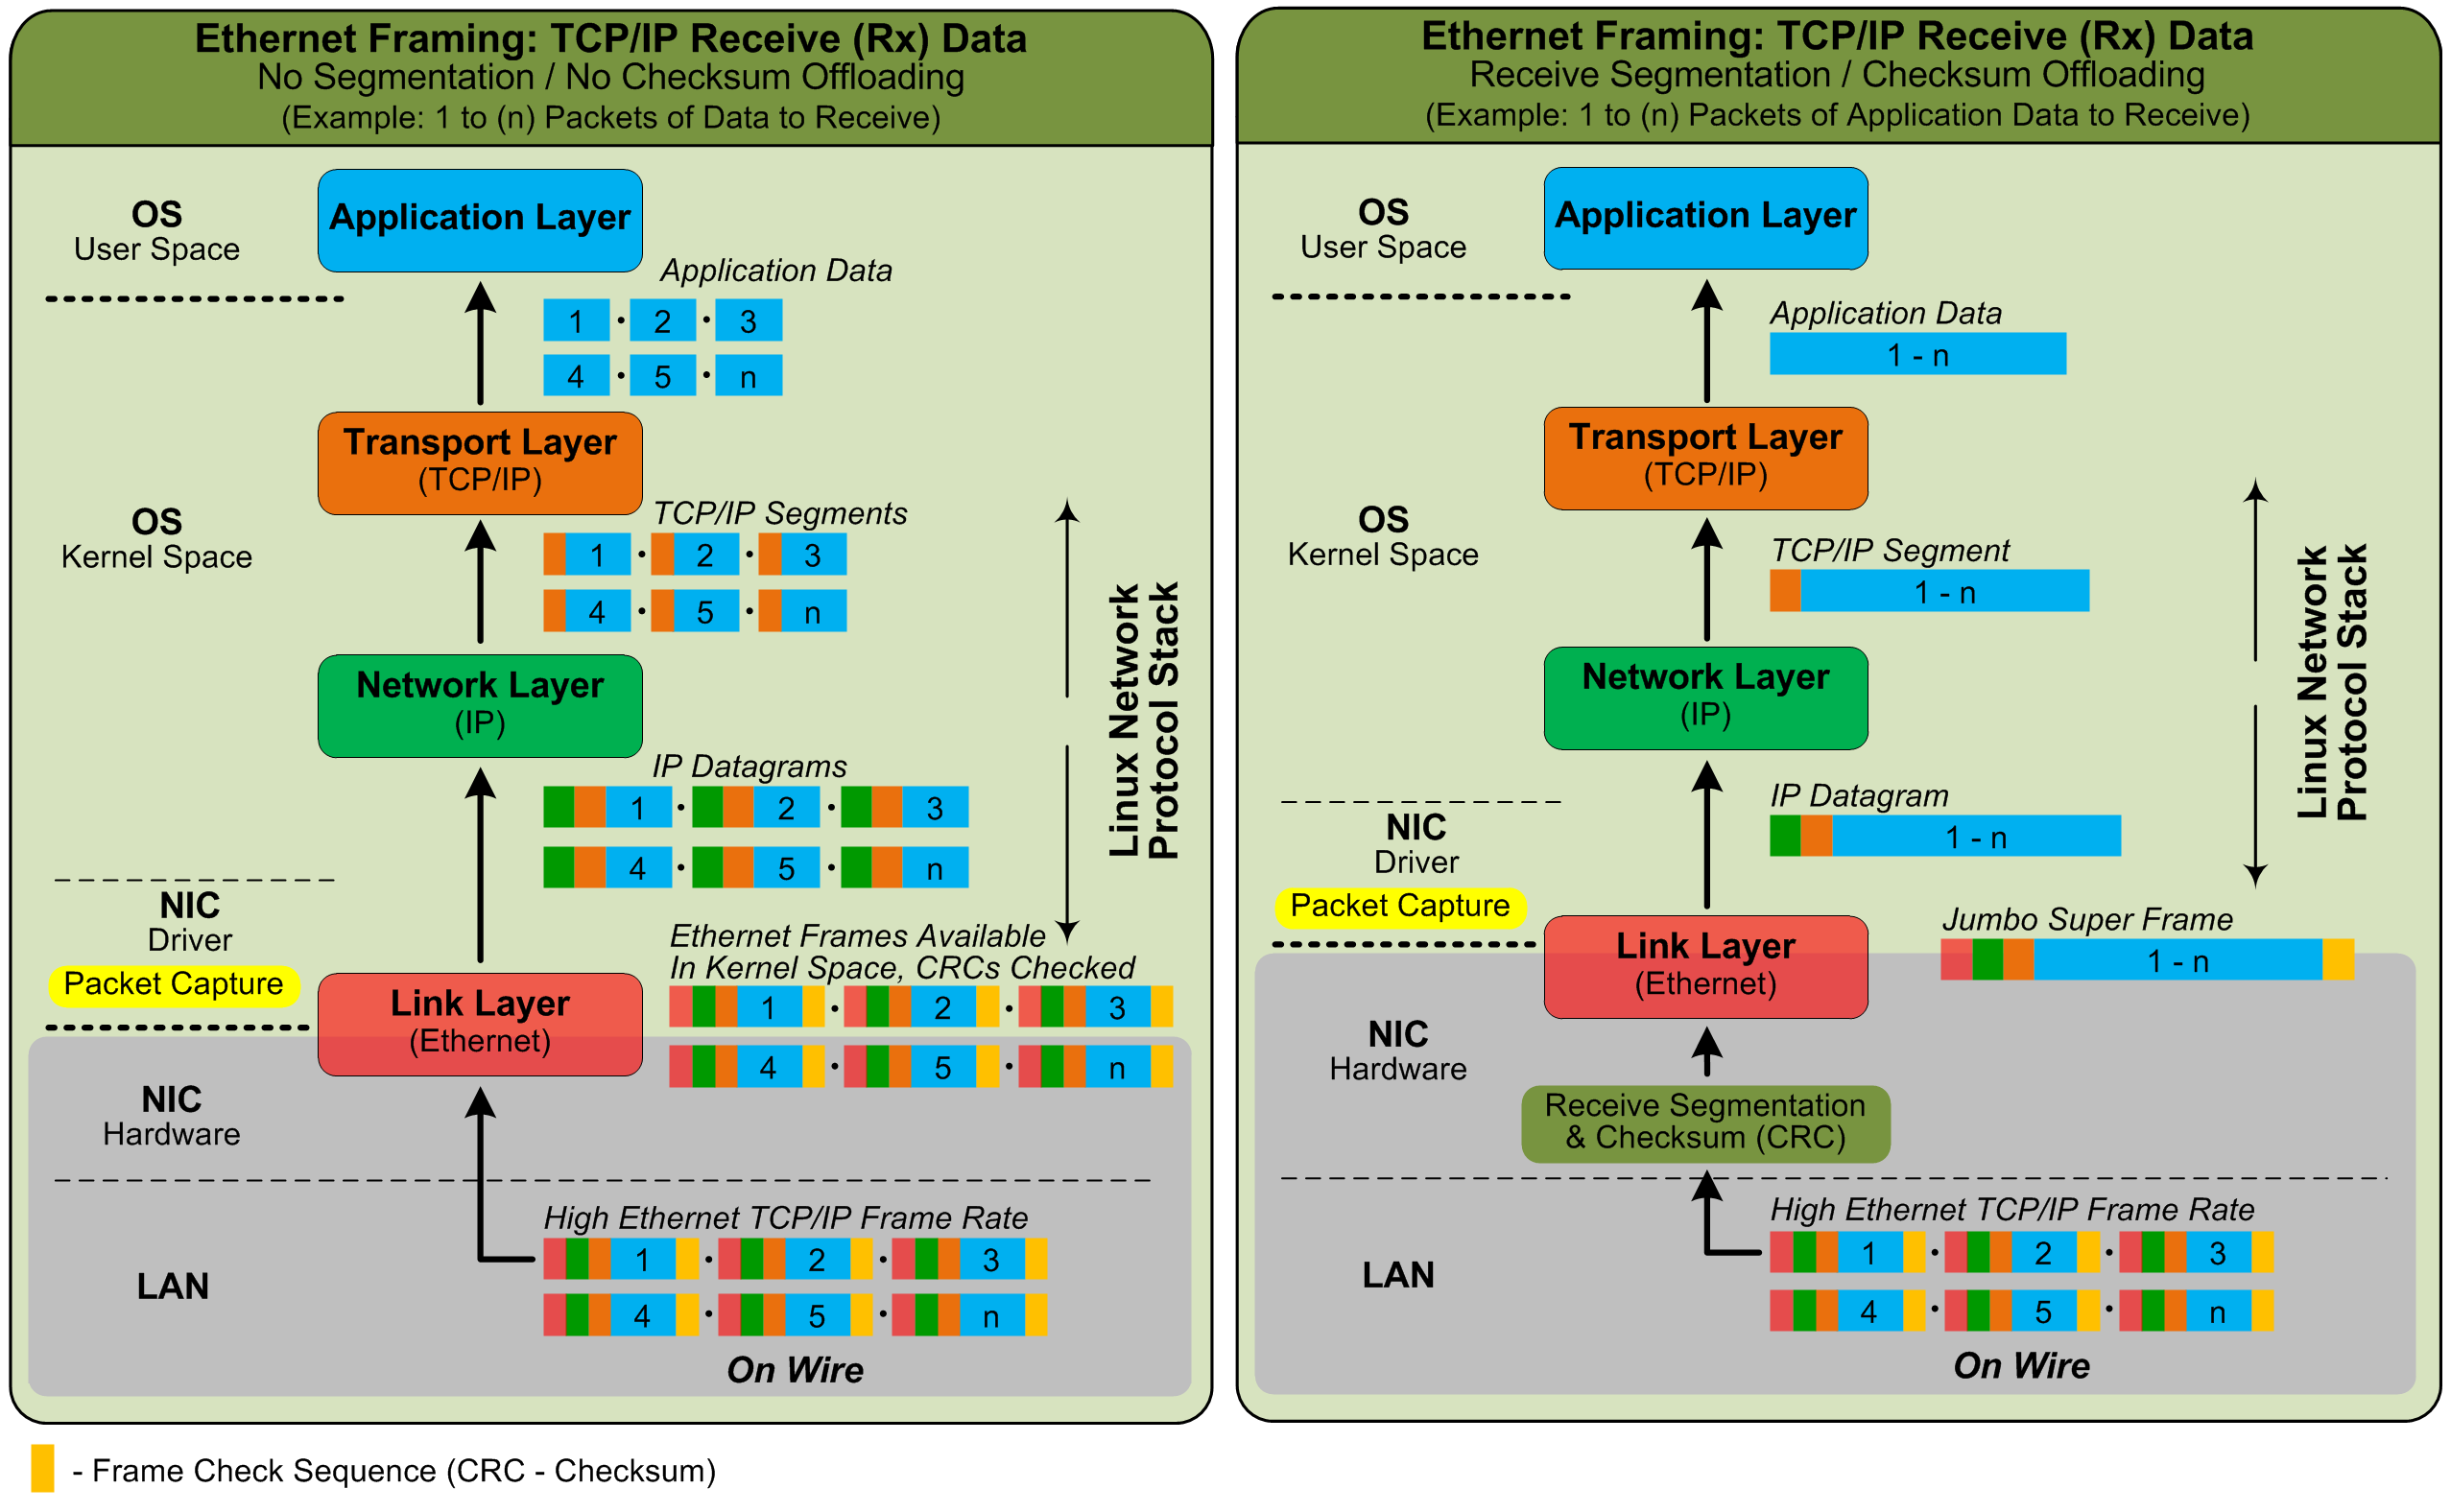
\includegraphics[width=15cm,keepaspectratio]{fig/rcv-offloads.png}
	\caption{Receive offloads (source:~\cite{nst-offloads})}
	\label{fig:linux-rcv-offloads}
	\bigskip
\end{figure}
